Let $(X, \rho)$ be a metric space. Let $\B$ be the family of bounded sets in $X$.

\begin{definition}\label{def:noncompactness_measures}(\cite[definition 7.1]{Deimling1985})
  We define the following functions
  \begin{defenum}
    \item\label{def:noncompactness_measures/sets} The \uline{Kuratowski measure of noncompactness},
    \begin{align*}
      &\alpha: \B \to \RPos \\
      &\alpha(A) \coloneqq \inf \{d > 0 \colon \exists U_1, \ldots, U_n \subseteq X: \Diam {U_k} < d \land A \subseteq \cup_{k=1}^n U_k \}
    \end{align*}

    \item\label{def:noncompactness_measures/balls} The \uline{ball measure of noncompactness},
    \begin{align*}
      &\beta: \B \to \RPos \\
      &\beta(A) \coloneqq \inf \{r > 0 \colon \exists x_1, \ldots, x_2 \in X: A \subseteq \cup_{k=1}^n B(x_k, r) \}
    \end{align*}
  \end{defenum}
\end{definition}

\begin{example}\label{ex:noncompactness_measures}(\cite[exercise 7.3]{Deimling1985})
  Consider the subsets $A_2 \subseteq A_3 \subseteq A_1 \subseteq C([0, 1])$, defined by
  \begin{align*}
    A_1 \coloneqq \left\{
      x \in C([0, 1]) \colon \begin{aligned}
        0 \leq t \leq 1 \implies 0 \leq x(t) \leq 1 \\
        x(0) = 0, x(1) = 1 \\
      \end{aligned}
    \right\}
    \\
    A_2 \coloneqq \left\{
      x \in A_1 \colon \begin{aligned}
        0 \leq t \leq \frac 1 2 \implies 0 \leq x(t) \leq \frac 1 2 \\
        \frac 1 2 \leq t \leq 1 \implies \frac 1 2 \leq x(t) \leq 1
      \end{aligned}
    \right\}
    \\
    A_3 \coloneqq \left\{
      x \in A_1 \colon \begin{aligned}
        0 \leq t \leq \frac 1 2 \implies 0 \leq x(t) \leq \frac 2 3 \\
        \frac 1 2 \leq t \leq 1 \implies \frac 1 3 \leq x(t) \leq 1
      \end{aligned}
    \right\}
  \end{align*}

  Then $\alpha(A_1) = 1, \alpha(A_2) = \frac 1 2, \alpha(A_3) = \frac 1 3$ and $\beta(A_1) = \beta(A_2) = \beta(A_3) = \frac 1 2$.
\end{example}
\begin{proof}
  Since the distance between any two functions from $B_1$ is at most 1, we have that $\Diam B_1 = 1$ and $\alpha(B_1) \leq 1$.

  Fix $\varepsilon > 0$. For any function $f \in B_1$, continuity of $f$ gives us a radius $\delta_f > 0$ such that
  \begin{align*}
    x < 2 \delta_f \implies f(x) < \varepsilon.
  \end{align*}

  \begin{figure}[ht]
    \begin{center}
      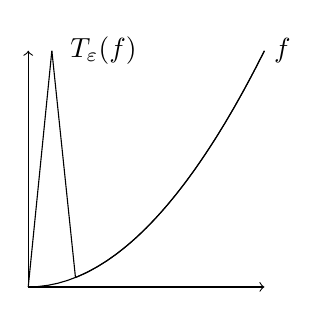
\begin{tikzpicture}[scale=3]
        \draw[->] (0, 0) -- (1, 0);
        \draw[->] (0, 0) -- (0, 1);

        \draw[domain=0:1, variable=\x] plot ({\x}, {\x^2}) node[right] {$f$};

        \draw (1/2, 1) node[left] {$T_\varepsilon(f)$};
        \draw[domain=0:0.1, variable=\x] plot ({\x}, {10 * \x});
        \draw[domain=0.1:0.2, variable=\x] plot ({\x}, {0.04 + (1 - 0.04) * (2 - 10 * \x)});
        \draw[domain=0.2:1, variable=\x] plot ({\x}, {\x^2});
      \end{tikzpicture}
    \end{center}
  \end{figure}

  Define
  \begin{align*}
    T_\varepsilon(f)(x) \coloneqq \begin{cases}
      \frac x \delta_f, &0 \leq x < \delta_f \\
      f(\delta_f) + [1 - f(\delta_f)] (2 - \frac x {\delta_f}), &\delta_f \leq x < 2 \delta_f \\
      f(x), &x \geq 2 \delta_f,
    \end{cases}
  \end{align*}
  so that
  \begin{align*}
    \Norm{T_\varepsilon(f) - f}
    \geq
    T_\varepsilon(f) (\delta_f) - f(\delta_f)
    =
    1 - f(\delta_f)
    >
    1 - \varepsilon.
  \end{align*}

  Additionally, because $\delta_{T_\varepsilon(f)} < \delta_f$, we have that $f(\delta_{T_\varepsilon(f)}) < \varepsilon$ and
  \begin{align*}
    \Norm{T_\varepsilon(T_\varepsilon(f)) - f}
    \geq
    T_\varepsilon(T_\varepsilon(f)) (\delta_{T_\varepsilon(f)}) - f(\delta_{T_\varepsilon(f)})
    =
    1 - f(\delta_{T_\varepsilon(f)})
    >
    1 - \varepsilon.
  \end{align*}

  Thus, proceeding by induction, we see that for any $m = 1, 2, \ldots$
  \begin{align*}
    \Norm{T_\varepsilon^m(f) - f} > 1 - \varepsilon,
  \end{align*}
  where $T_\varepsilon^m$ denotes repeated application of $T_\varepsilon$.

  Consider the sequence
  \begin{align*}
    \{ T_\varepsilon^k(f) \}_{k=0}^\infty = \{ f, T_\varepsilon(f), T_\varepsilon(T_\varepsilon(f)), \ldots \}.
  \end{align*}

  We can easily see that the distance between any two elements of the sequence, say $T_\varepsilon^k(f)$ and $T_\varepsilon^{k+m}(f)$, is strictly greater that $1 - \varepsilon$, i.e.
  \begin{align*}
    \Norm{T_\varepsilon^k(f) - T_\varepsilon^{k+m}(f)}
    =
    \Norm{T_\varepsilon^k(f) - T_\varepsilon^m(T_\varepsilon^k(f))}
    >
    1 - \varepsilon.
  \end{align*}

  Hence $B_1$ cannot be covered by a finite $(1-\varepsilon)$-net and $\alpha(B_1) \geq 1 - \varepsilon$. Since $\varepsilon > 0$ can be made arbitrarily small, this implies that $\alpha(B_1) \geq 1$ and, because we already have the reverse inequality, $\alpha(B_1) = 1$.

  In the set $B_2$, the maximum distance between two functions is $\frac 1 2$, thus $\Diam(B_2) = \frac 1 2$ and $\alpha(B_2) \leq \frac 1 2$. We can then define an operator similar to $T_\varepsilon$ that creates \enquote{spikes} of height $\frac 1 2$ to prove the reverse inequality, obtaining
  \begin{align*}
    \alpha(B_2) = \frac 1 2.
  \end{align*}

  Finally, the set $B_3$ has diameter $\frac 2 3$ and hence $\alpha(B_3) = \frac 2 3$.

  The ball measure for $B_1$ satisfies the inequalities
  \begin{align*}
    \frac 1 2 \leq \beta(B_1) \leq 1.
  \end{align*}

  Additionally, $B_1$ is strictly contained in the ball centered in the constant function $\frac 1 2$ with radius $\frac 1 2$, which implies that $\beta(B_1) \leq \frac 1 2$, hence $\beta(B_1) = \frac 1 2$.

  For $B_2$ we have
  \begin{align*}
    \frac 1 4 \leq \beta(B_2) \leq \frac 1 2.
  \end{align*}

  Assume\LEM that for some $\varepsilon > 0$ the set $B_2$ can be covered by a finite set of balls with centers $\{ f_1, \ldots, f_n \} \subsetneq C([0, 1])$ and radius $\frac 1 2 - \varepsilon$.

  Because of continuity, we can find a radius $\delta > 0$ such that for all $f_k, k = 1, \ldots, n$ we have
  \begin{align*}
    x \in \left[\tfrac {1 - \delta} 2, \tfrac {1 + \delta} 2 \right] \implies \Abs{f_k(x) - f_k(\tfrac 1 2)} < \varepsilon.
  \end{align*}

  Consider the function
  \begin{align*}
    g(x) \coloneqq \begin{cases}
      0, &0 \leq x < \frac {1 - \delta} 2, \\
      \frac{2x + \delta - 1} {2\delta}, &\frac {1 - \delta} 2 \leq x \leq \frac {1 + \delta} 2, \\
      1, &\frac {1 + \delta} 2 < x \leq 1.
    \end{cases}
  \end{align*}

  \begin{figure}[ht]
    \begin{center}
      \begin{tikzpicture}[scale=5]
        \draw[->] (0, 0) -- (1, 0);
        \draw[->] (0, 0) -- (0, 1);
        \draw[domain=0:4/10, thick, variable=\x] plot ({\x}, {0});
        \draw[domain=4/10:6/10, thick, variable=\x] plot ({\x}, {5 * \x - 2}) node[left] {$g$};
        \draw[domain=6/10:1, thick, variable=\x] plot ({\x}, {1});

        \draw[densely dotted] (0, 6/10) node[left] {$f_k(\frac 1 2) - \varepsilon$} -- (1, 6/10);
        \draw[densely dotted] (0, 8/10) node[left] {$f_k(\frac 1 2) + \varepsilon$} -- (1, 8/10);

        \draw[densely dotted] (4/10, 0) -- (4/10, 1);
        \draw (3/10, -1/10) node {$\frac {1 - \delta} 2$};
        \draw[densely dotted] (1/2, 0) -- (1/2, 1);
        \draw (1/2, -1/10) node {$\frac 1 2$};
        \draw[densely dotted] (6/10, 0) -- (6/10, 1);
        \draw (7/10, -1/10) node {$\frac {1 + \delta} 2$};

        \draw[domain=-1/10:1, dash dot, variable=\x] plot ({\x}, {2/10 + 1 / (1 + e^(5/3*(1-2*\x)))}) node[right] {$f_k$};
      \end{tikzpicture}
    \end{center}
  \end{figure}

  If $f_k(\tfrac 1 2) \geq \frac 1 2$, then $f_k(\tfrac {1 - \delta} 2) > \tfrac 1 2 - \varepsilon$ and
  \begin{align*}
    \Norm{f_k - g} \geq f_k(\tfrac {1 - \delta} 2) - g(\tfrac {1 - \delta} 2) = f_k(\tfrac {1 - \delta} 2) > \tfrac 1 2 - \varepsilon.
  \end{align*}

  Analogously, if $f_k(\tfrac 1 2) < \frac 1 2$, then $f_k(\tfrac {1 + \delta} 2) < \tfrac 1 2 + \varepsilon$ and
  \begin{align*}
    \Norm{g - f_k} \geq g(\tfrac {1 + \delta} 2) - f_k(\tfrac {1 + \delta} 2) = 1 - f_k(\tfrac {1 + \delta} 2) > \tfrac 1 2 - \varepsilon.
  \end{align*}

  Thus, for every $k = 1, \ldots, n$ we have
  \begin{align*}
    \Norm{g - f_k} > \frac 1 2 - \varepsilon,
  \end{align*}
  i.e. $g$ in not contained in a ball of radius $\frac 1 2 - \varepsilon$ around any of the centers $f_1, \ldots, f_n$.

  Hence $\beta(B_2) \geq \frac 1 2$, which implies $\beta(B_2) = \frac 1 2$. Because of the inclusion $B_2 \subsetneq B_3 \subsetneq B_1$, we have
  \begin{align*}
    \frac 1 2 = \beta(B_2) \leq \beta(B_3) \leq \beta(B_1) = \frac 1 2,
  \end{align*}
  hence $\beta(B_3) = \frac 1 2$.
\end{proof}

\begin{theorem}\label{thm:noncompact_kuratowski_lemma}(\cite[exercise 7.4]{Deimling1985}, Kuratowski lemma)
  Let $X$ be a Banach space and $\{ A_n \}_n$ be a decreasing sequence of nonempty closed subsets such that $\alpha(A_n) \to 0$. Then $A \coloneqq \bigcap_n A_n$ is nonempty and compact.
\end{theorem}
\begin{proof}
  The set $A$ is compact because it is closed as the intersection of closed sets and $\alpha(A) \leq \alpha(A_n) \to 0$, hence $\alpha(A) = 0$.

  It remains to show that $A$ is nonempty.
  Choose\AOC any sequence $\{ x_n \}_n$ where $x_n \in A_n$. Since any finite set is compact, we have that for any $k \geq 1$
  \begin{align*}
    \alpha(\{ x_n \}_{n \geq 1})
    =
    \max\{ \alpha(\{ x_n \}_{n < k}), \alpha(\{ x_n \}_{n \geq k}) \}
    =
    \alpha(\{ x_n \}_{n \geq k})
    \leq
    \alpha(A_k) \to 0,
  \end{align*}
  hence the set $\{ x_n \colon n \geq 1 \}$ is compact and thus sequentially compact. We can choose a convergent subsequence $\{ x_{n_k} \}_k$ of $\{ x_n \}_n$ whose limit lies in every $A_n$ (since they are closed) and, consequently, in their intersection $A$. So $A$ is nonempty.
\end{proof}
